% The official USENIX style is supplied unchanged in usenix2019_v3.sty.
\begin{filecontents*}{usenix2019_v3.sty}
% usenix.sty - to be used with latex2e for USENIX.
% To use this style file, look at the template usenix_template.tex
%
% $Id: usenix.sty,v 1.2 2005/02/16 22:30:47 maniatis Exp $
%
% The following definitions are modifications of standard article.sty
% definitions, arranged to do a better job of matching the USENIX
% guidelines.
% It will automatically select two-column mode and the Times-Roman
% font.
%
% 2018-12-19 [for ATC'19]: add packages to help embed all fonts in
%   pdf; to improve appearance (hopefully); to make refs and citations
%   clickable in pdf

%
% USENIX papers are two-column.
% Times-Roman font is nice if you can get it (requires NFSS,
% which is in latex2e.

\if@twocolumn\else\input twocolumn.sty\fi
\usepackage{mathptmx}  % times roman, including math (where possible)

% hopefully embeds all fonts in pdf
\usepackage[T1]{fontenc}
\usepackage[utf8]{inputenc}
\usepackage{pslatex}

% appearance
\usepackage[kerning,spacing]{microtype} % more compact and arguably nicer
\usepackage{flushend} % make cols in last page equal in size

% refs and bib
\usepackage{cite}               % order multiple entries in \cite{...}
\ifdefined\XeTeXrevision\else
\usepackage{breakurl}           % break too-long urls in refs (pdfTeX)
\fi
\usepackage{url}                % allow \url in bibtex for clickable links
\usepackage{xcolor}             % color definitions, to be use for...
\usepackage[]{hyperref}         % ...clickable refs within pdf...
\hypersetup{                    % ...like so
  colorlinks,
  linkcolor={green!80!black},
  citecolor={red!70!black},
  urlcolor={blue!70!black}
}

%
% USENIX wants margins of: 0.75" sides, 1" bottom, and 1" top.
% 0.33" gutter between columns.
% Gives active areas of 7" x 9"
%
\setlength{\textheight}{9.0in}
\setlength{\columnsep}{0.33in}
\setlength{\textwidth}{7.00in}

\setlength{\topmargin}{0.0in}

\setlength{\headheight}{0.0in}

\setlength{\headsep}{0.0in}

\addtolength{\oddsidemargin}{-0.25in}
\addtolength{\evensidemargin}{-0.25in}

% Usenix wants no page numbers for camera-ready papers, so that they can
% number them themselves.  But submitted papers should have page numbers
% for the reviewers' convenience.
%
%
% \pagestyle{empty}

%
% Usenix titles are in 14-point bold type, with no date, and with no
% change in the empty page headers.  The whole author section is 12 point
% italic--- you must use {\rm } around the actual author names to get
% them in roman.
%
\def\maketitle{\par
 \begingroup
   \renewcommand\thefootnote{\fnsymbol{footnote}}%
   \def\@makefnmark{\hbox to\z@{$\m@th^{\@thefnmark}$\hss}}%
    \long\def\@makefntext##1{\parindent 1em\noindent
            \hbox to1.8em{\hss$\m@th^{\@thefnmark}$}##1}%
   \if@twocolumn
     \twocolumn[\@maketitle]%
     \else \newpage
     \global\@topnum\z@
     \@maketitle \fi\@thanks
 \endgroup
 \setcounter{footnote}{0}%
 \let\maketitle\relax
 \let\@maketitle\relax
 \gdef\@thanks{}\gdef\@author{}\gdef\@title{}\let\thanks\relax}

\def\@maketitle{\newpage
 \vbox to 2.5in{
 \vspace*{\fill}
 \vskip 2em
 \begin{center}%
  {\Large\bf \@title \par}%
  \vskip 0.375in minus 0.300in
  {\large\it
   \lineskip .5em
   \begin{tabular}[t]{c}\@author
   \end{tabular}\par}%
 \end{center}%
 \par
 \vspace*{\fill}
% \vskip 1.5em
 }
}

%
% The abstract is preceded by a 12-pt bold centered heading
\def\abstract{\begin{center}%
{\large\bf \abstractname\vspace{-.5em}\vspace{\z@}}%
\end{center}}
\def\endabstract{}

%
% Main section titles are 12-pt bold.  Others can be same or smaller.
%
\def\section{\@startsection {section}{1}{\z@}{-3.5ex plus-1ex minus
    -.2ex}{2.3ex plus.2ex}{\reset@font\large\bf}}
\end{filecontents*}
\documentclass[letterpaper,twocolumn,10pt]{article}
\ifdefined\XeTeXrevision
  \usepackage{hyperref}
\fi
\usepackage{usenix2019_v3}
\ifdefined\XeTeXrevision
  \microtypesetup{spacing=false,kerning=false}
\fi
\usepackage{amsmath}
\usepackage{array}
\usepackage{booktabs}
\usepackage{tikz}
\usetikzlibrary{arrows.meta}

\begin{document}
\date{}
\title{\Large \bf MASGuardEval: Risk-Aware Evaluation and Failure Tracing for Multi-Agent Systems}
\author{Anonymous Submission}
\maketitle

\begin{abstract}
A multi-agent system can complete a user request while an intermediate agent crosses an authorization boundary, leaks information, or passes a faulty instruction to another agent. A final task score does not identify the initiating event or show whether the fault spread. We present MASGuardEval, an implemented software-workspace framework that records agent and tool events as structured spans, projects observed interactions into a directed agent--tool graph, computes risk-oriented trace measures, and executes matched unguarded and guarded runs in isolated task environments. The system links messages, tool calls, blocked attempts, and parent-span dependencies to an inspectable timeline and graph. It includes scenario review, trace persistence, outcome-review packets, and held-out analysis tools. We exercise the full runner with seven reference scenarios and a pinned local model in single-agent and Planner--Executor--Reviewer configurations; 13 of 14 recorded baseline/guarded pairs are protocol valid. These observations verify an executable evaluation path and expose one adapter protocol error. They do not establish independent diagnostic accuracy or a safety improvement.
\end{abstract}

\section{Introduction}
\label{sec:introduction}

Consider a software-workspace task in which a planner asks an executor to update a configuration file and a reviewer later reports completion. If the planner supplied a faulty instruction, the executor wrote an unauthorized change, and the reviewer accepted it, the final response alone gives a poor account of the failure. Evaluation needs to identify the instruction, the agent or tool boundary at which it mattered, the subsequent actions, and the resulting workspace state. Figure~\ref{fig:motivation} illustrates the event sequence and the evidence a final-answer score omits.

\begin{figure*}[t]
\centering
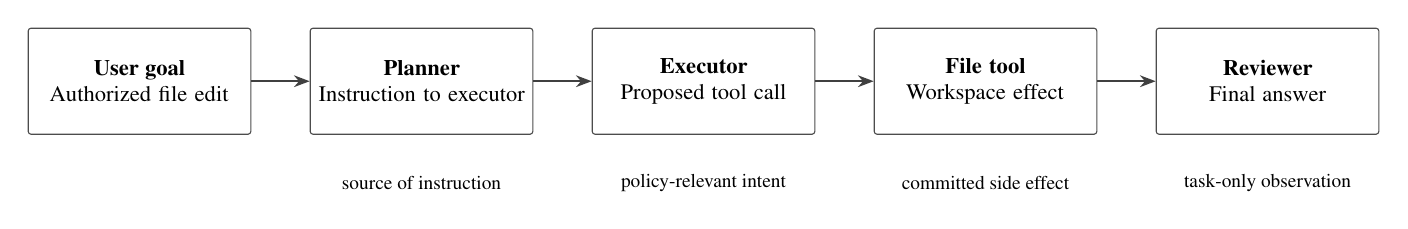
\begin{tikzpicture}[x=1in,y=1in,
  trace/.style={draw=black!70,rounded corners=1pt,align=center,
    text width=1.03in,minimum height=.53in,inner sep=3pt,font=\footnotesize},
  link/.style={-Stealth,semithick,draw=black!75}]
\node[trace] (goal) at (.60,0) {\textbf{User goal}\\Authorized file edit};
\node[trace] (plan) at (2.01,0) {\textbf{Planner}\\Instruction to executor};
\node[trace] (intent) at (3.42,0) {\textbf{Executor}\\Proposed tool call};
\node[trace] (effect) at (4.83,0) {\textbf{File tool}\\Workspace effect};
\node[trace] (answer) at (6.24,0) {\textbf{Reviewer}\\Final answer};
\draw[link] (goal) -- (plan);
\draw[link] (plan) -- (intent);
\draw[link] (intent) -- (effect);
\draw[link] (effect) -- (answer);
\node[font=\scriptsize,align=center] at (2.01,-.51) {source of instruction};
\node[font=\scriptsize,align=center] at (3.42,-.51) {policy-relevant intent};
\node[font=\scriptsize,align=center] at (4.83,-.51) {committed side effect};
\node[font=\scriptsize,align=center] at (6.24,-.51) {task-only observation};
\end{tikzpicture}
\caption{Illustrative multi-agent trace, not a pilot result. If the proposed file operation exceeds the user's authorization, a final-answer score cannot identify the initiating instruction, the tool boundary, or the committed side effect. MASGuardEval retains the event spans and their observed links for inspection.}
\label{fig:motivation}
\end{figure*}

Tool-using agents make this problem concrete. An agent's output can become another agent's input or a tool invocation with a side effect. An exploratory live study documented unsafe tool behavior and multi-party failures~\cite{shapira2026chaos}. Benchmark environments separate legitimate task success from adversarial outcomes~\cite{debenedetti2024agentdojo,ruan2024toolemu}, while recent work addresses failure localization and multi-agent telemetry~\cite{barke2026agentrx,seyedghorban2026observability,balusu2026agenttelemetry}. MASGuardEval brings these questions into one trace-linked evaluation workflow: component and path diagnosis, risk measurement, and matched mitigation comparison.

MASGuardEval runs tool-using single-agent and Planner--Executor--Reviewer workflows against an isolated software workspace. It records typed spans, projects agent--tool relations and executed graph routes into an observed graph, calculates eight operational trace measures, and supports paired unguarded and guarded runs. Guards act as pre-execution interventions; a block prevents the proposed tool effect but may also prevent legitimate completion.

MASGuardEval organizes evaluation around three questions. \emph{RQ1 (diagnosis):} Which risky event, agent or tool, and downstream trace path explain a failure? \emph{RQ2 (measurement):} Which trace measures remain informative when compared with independent judgments and held-out task families? \emph{RQ3 (mitigation):} How do targeted guards change prohibited actions, legitimate completion, and execution cost in matched runs? The implementation generates structured traces, candidate graph paths, metric scores, and paired-run records for these analyses. Section~\ref{sec:pilot} reports the evidence actually collected.

\noindent\textbf{Contributions.} The paper presents (1) a controlled evaluation pipeline that separates proposed actions, blocked attempts, and committed effects; (2) a span-linked graph of agent--tool interactions and executed workflow routes, a visual explorer, and eight operational trace measures; and (3) a common execution boundary for paired mitigation conditions. The design connects failure tracing to mitigation benchmarking while keeping graph provenance separate from causal proof and guard stops separate from task success.

\section{Literature survey}
\label{sec:related}

Prior work addresses three connected questions: which agent behaviors create risk, what trace evidence can identify a failure, and whether an intervention prevents harm while preserving the authorized task. The studies below inform the evaluation design and delimit what its pilot can claim.

\paragraph{Risk settings and executable benchmarks.}
\emph{Agents of Chaos} reports eleven case studies from a two-week live-agent laboratory. Its observed failures include unauthorized compliance, disclosure, resource consumption, and unsafe behavior spreading between agents; in some cases, completion reports disagreed with system state~\cite{shapira2026chaos}. These observations motivate checking tool effects and cross-agent sequences, but the present isolated workspace cannot reproduce the laboratory's deployment conditions. AgentDojo supplies an extensible tool-use environment with legitimate tasks, attacker objectives, and prompt-injection attacks and defenses~\cite{debenedetti2024agentdojo}. It shows why task completion and security outcomes must be assessed separately. ToolEmu instead emulates tools with a language model to explore risky actions at scale and uses human evaluation to check identified failures~\cite{ruan2024toolemu}. MASGuardEval uses deterministic mock tool effects so each proposed action can be compared with an observed workspace change. This favors execution auditability over ToolEmu's breadth of emulated tools and scenarios.

\paragraph{Failure localization and telemetry.}
AgentRx releases annotated failed trajectories and localizes a critical failure step using constraint checks and an evidence log~\cite{barke2026agentrx}. Its independently annotated localization task is a stronger diagnostic test than displaying a plausible failure path. The framework-agnostic llmmas-otel combines multi-agent traces with targeted fault injection and aligned baseline/faulty runs in software-engineering workflows~\cite{seyedghorban2026observability}. AgentTelemetry defines agent-specific span kinds and evaluates fault detectability under different observability conditions~\cite{balusu2026agenttelemetry}. These works show that both evidence coverage and independent labels matter. MASGuardEval links agent and tool spans to a graph, trace measures, and saved workspace effects, but its graph roots rely partly on recorded annotations. The pilot therefore demonstrates inspectability rather than measured root-cause accuracy.

\paragraph{Runtime controls and action attribution.}
NeMo Guardrails' execution rails validate tool calls, arguments, and results at the tool boundary~\cite{nvidia2026rails}. AttriGuard targets indirect prompt injection more specifically: it re-evaluates a proposed tool action under altered external observations and gates actions whose support does not survive that counterfactual test~\cite{he2026attriguard}. MASGuardEval supplies simpler policy checks before mock execution. It records the rejected intent as well as permitted effects, which lets a reviewer distinguish a stopped attempt from a completed legitimate task. Its current checks should not be read as equivalent to AttriGuard's causal-attribution defense.

\paragraph{Position of this work.}
Across these studies, realistic failure cases, dynamic task evaluation, trace-based diagnosis, and tool-boundary defenses are well established. MASGuardEval's contribution is the common, span-linked record used to inspect a controlled task, an agent--tool projection, operational risk measures, and matched guarded and unguarded executions. That integration supports a reproducible workflow; comparative gains in diagnosis or safety require independent outcome labels and a larger held-out study.

\section{Problem and scope}
\label{sec:problem}

\subsection{Tasks, events, and outcomes}

A scenario specifies a legitimate user goal, role and policy context, permitted and prohibited actions, tool schemas, initial workspace state, and a rubric for successful authorized behavior. A run is one execution of an agent architecture on one scenario under one configuration. Let $T=(s_1,\ldots,s_n)$ be its ordered spans. A span can describe an agent step, inter-agent message, proposed or executed tool call, guard decision, memory operation, or final response. Each span can include an identifier, parent identifier, acting agent, tool, timestamp, input or output, policy decision, and optional failure annotation.

We distinguish four outcomes. A \emph{prohibited attempt} is an agent's proposed action that violates the scenario policy. A \emph{committed prohibited action} is a prohibited action that reached the mock executor and changed or exposed workspace state. A \emph{blocked attempt} is visible in the trace but produced no tool side effect. \emph{Legitimate completion} is fulfillment of the authorized task according to an independent rubric. The runner records adapter protocol errors separately, even when they cause task failure. Outcome-review tooling keeps a guard decision or metric threshold separate from an independently judged task outcome.

The reference dataset spans unauthorized compliance, sensitive-data disclosure, tool misuse, infinite looping, cascading failure, context pollution, and contradictory coordination. These are selected software-workspace risks, not a universal taxonomy. Seven reference scenarios exercise the runner and dashboard. A separate collection of 35 generated candidate variants is synthetic and is excluded from the pilot results reported here.

\subsection{Graph meaning and attribution limits}

MASGuardEval constructs a directed observed graph $G=(V,E)$. Agent and tool nodes are linked by reached tool calls, inter-agent messages, selected cross-agent control flow, and blocked or approval-required attempts. For instrumented LangGraph runs, separate graph-node vertices and transition edges record the executed route, including nested graph namespaces; unchosen static branches are not recorded as executed. Runtime spans also record checkpoint identifiers and interrupt or resume events. Every displayed edge refers to a source span. At span level, the implementation keeps structural parent links separate from declared dependency links. The latter resolve an adapter's \texttt{caused\_by} event reference to a recorded source span; missing or ambiguous references do not create dependency edges. A saved trace may also carry an explicit source span ID. Candidate failure paths follow only these declared links, possibly through intermediate spans without failure labels.

These edges are \emph{observational provenance}. An earlier parent span may be relevant to a later failure without being its cause, and missing instrumentation can omit a dependency. The candidate causal span graph uses declared dependencies rather than treating nesting as influence. A root is a failure-labelled span with no earlier failure along those links; a downstream failure is connected to such a root by a declared path. A \texttt{propagated\_from} annotation without a supported path is reported as unlinked instead of being counted as propagation. Each displayed root or path is trace evidence for inspection, not an independently established causal claim. The graph retains source span identifiers so an analyst can inspect the event sequence and assess competing explanations.

The threat model includes agents that misinterpret a legitimate request, follow untrusted context, violate role or parameter constraints, loop, or pass a faulty instruction to another agent. Policies and task rubrics are supplied by the evaluation scenario; agent text and tool-returned text are lower-trust inputs. The mock executor confines email, file, memory, job, and simulated shell actions to a fresh in-memory workspace. This supports controlled tests of policy-relevant behavior but does not reproduce all permissions, races, or side effects of external services.

\section{MASGuardEval design}
\label{sec:design}

\begin{figure*}[t]
\centering
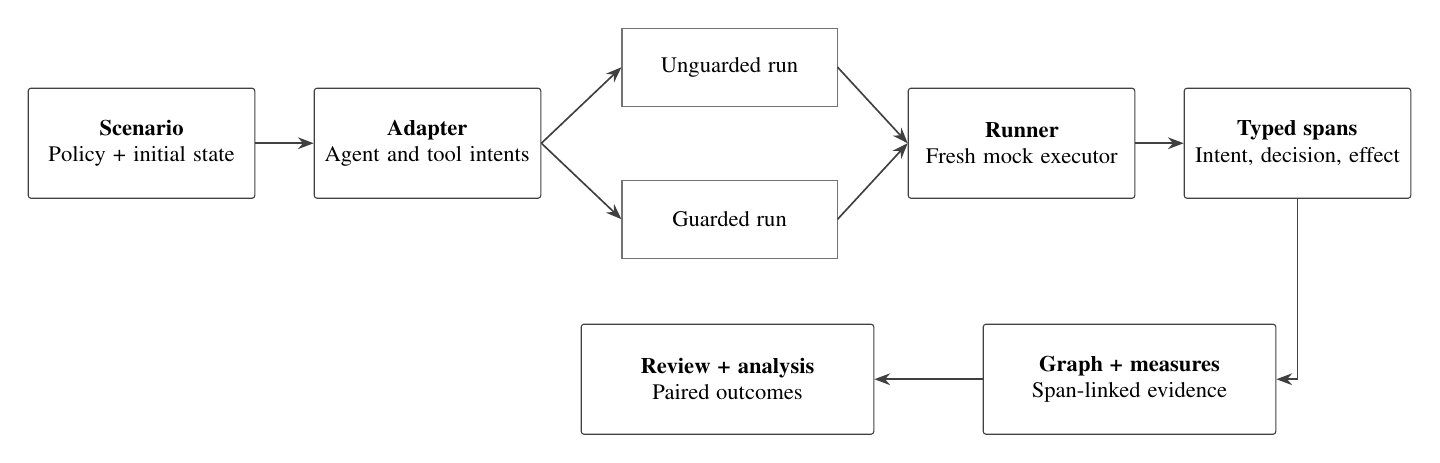
\begin{tikzpicture}[x=1in,y=1in,
  stage/.style={draw=black!75,rounded corners=1pt,align=center,
    text width=1.05in,minimum height=.55in,inner sep=3pt,font=\footnotesize},
  condition/.style={draw=black!55,align=center,text width=1.02in,
    minimum height=.39in,inner sep=2pt,font=\footnotesize},
  link/.style={-Stealth,semithick,draw=black!75}]
\node[stage] (scenario) at (.62,0) {\textbf{Scenario}\\Policy + initial state};
\node[stage] (adapter) at (2.05,0) {\textbf{Adapter}\\Agent and tool intents};
\node[condition] (base) at (3.56,.38) {Unguarded run};
\node[condition] (guard) at (3.56,-.38) {Guarded run};
\node[stage] (runner) at (5.02,0) {\textbf{Runner}\\Fresh mock executor};
\node[stage] (spans) at (6.40,0) {\textbf{Typed spans}\\Intent, decision, effect};
\draw[link] (scenario) -- (adapter);
\draw[link] (adapter.east) -- (base.west);
\draw[link] (adapter.east) -- (guard.west);
\draw[link] (base.east) -- (runner.west);
\draw[link] (guard.east) -- (runner.west);
\draw[link] (runner) -- (spans);
\node[stage,text width=1.38in] (graph) at (5.56,-1.18) {\textbf{Graph + measures}\\Span-linked evidence};
\node[stage,text width=1.38in] (review) at (3.55,-1.18) {\textbf{Review + analysis}\\Paired outcomes};
\draw[link] (spans.south) |- (graph.east);
\draw[link] (graph) -- (review);
\end{tikzpicture}
\caption{Implemented evaluation path. Each condition starts from a fresh workspace. The guarded path checks an intent before tool execution; both paths produce typed spans. Span identifiers connect observed graph edges and measures to review records. The graph represents recorded relations, not independently established causation.}
\label{fig:pipeline}
\end{figure*}

\subsection{Controlled execution and capture}

An adapter chooses the next agent step or tool intent. The runner records the intent and, in guarded mode, evaluates applicable rules before calling a registered tool handler. Its checks cover failure isolation, coordination, role and attribute access, allowlists, parameters, context, repetition, and approval requirements. If a guard blocks or pauses a call, the trace records the decision and the downstream tool handler does not run. If the call proceeds, the actual mock result is recorded and returned to the adapter. Unguarded and guarded conditions begin with separate fresh workspace instances so one run's changes cannot carry into the other (Figure~\ref{fig:pipeline}). Only calls routed through this boundary are guarded and traced; an unwrapped tool or side effect within a graph node remains outside its control.

The default adapter is scripted and supports deterministic reference checks. Model-driven adapters support one controller or Planner--Executor--Reviewer roles. A bounded ReAct (reason--act) LangGraph subgraph obtains a model action at each reason node, routes reached tool calls through the guarded session, and feeds the observed result into the next reason node. The nested team graph runs Planner, Executor, and Reviewer subgraphs; the Reviewer either approves or routes to another bounded Executor round. A separate deterministic two-subgraph probe checks repeated routes and blocked branches without constituting a model-reasoning trial. The repeated-action guard blocks the same agent/action/tool pattern at its configured recent-history threshold (three by default); finite action-step, review-round, and graph-recursion budgets bound the model-driven paths. These mechanisms limit the implemented runs, not arbitrary agent loops.

The Python SDK registers systems, datasets, tools, and guards. Its custom-agent CLI can call a factory twice for fresh baseline and guarded adapter instances with isolated mock workspaces, then export both traces and per-condition evidence; unguarded execution requires explicit opt-in and isolated handlers. Native wrappers for LangChain, LangGraph, AutoGen, and CrewAI connect tool calls to the same guard boundary; local integration tests exercise their tool interfaces. LangGraph runtime observation records executed nodes, conditional routes, checkpoint identifiers, and interrupts or resumes without storing graph-state values in observation spans. SQLite persists runs and spans by default, reconstructs saved-run graphs, and streams new spans over the API. The implementation also includes a PostgreSQL JSONB store, a scenario index for caller-supplied pgvector embeddings, and explicit LangSmith run-tree export. These integrations were checked separately from the local-model pilot.

\subsection{Graph, measures, and inspection}

The graph builder uses span identifiers to connect agent--tool edges to underlying evidence. The dashboard displays the same saved trace as a timeline, graph, and metric comparison, including proposed and blocked intents, executed calls, stop reasons, and applicability flags. The reviewer can move from an aggregate score to its contributing spans and workspace effects. The system exposes candidate roots and paths; it does not replace an independent diagnosis.

Table~\ref{tab:metrics} defines seven secondary operational measures and one descriptive trace measure (DT). CFP is an observed trace share, not a population probability; DT is a normalized first-signal position, not elapsed analyst diagnosis time or a directional safety outcome. A zero-denominator measure is reported as not applicable rather than as zero risk. Several measures depend on adapter annotations, so their scores remain separate from independent outcome labels.

For Table~\ref{tab:metrics}, let $C$ be all tool-call spans, $U\subseteq C$ the unblocked calls, and $U^+\subseteq U$ those without a tool-execution-error label. The function $t(c)$ gives the tool named by call $c$, and $t(X)=\{t(c):c\in X\}$ for a set of calls $X$; $A$ and $R_T$ are the scenario's allowed and distinct required tool sets. Let $C_P\subseteq C$ contain calls assessed by a schema or explicit parameter label. Let $K_A$ contain context-bearing spans with an explicit Boolean pollution assessment, and $p(k)$ indicate one marked polluted but not sanitized. Let $F$ be failure-labeled spans excluding guard decisions and graph-observation spans (node, transition, checkpoint, and interrupt), and $R_F\subseteq F$ the roots without an earlier failure on a declared dependency path. The relation $r\prec f$ means that $f$ is reachable from $r$ through one or more declared span-dependency links; ordinary parent-span ancestry does not satisfy this relation. Finally, $S$ is the runtime-selected set of sensitive spans, $V\subseteq S$ its unauthorized spans that were neither blocked nor held for approval, $D_C$ is the set of decisions comparable on the same scope and revision, and $D_X\subseteq D_C$ contains decisions in a disagreeing group. These are trace-derived sets, not independent ground truth.

\begin{table*}[t]
\centering
{\renewcommand{\arraystretch}{1.18}
\begin{tabular}{@{}l>{\centering\arraybackslash}m{4.05in}>{\raggedright\arraybackslash}m{1.20in}c@{}}
\toprule
Key & Implemented score & N/A if & Better \\
\midrule
TSP & $\displaystyle\frac{\sum_{c\in U}\mathbf{1}[t(c)\in A]}{|U|}$ & $|U|=0$ & $\uparrow$ \\
TSR & $\displaystyle\frac{|R_T\cap t(U^+)|}{|R_T|}$ & $|R_T|=0$ & $\uparrow$ \\
PHR & $\displaystyle\frac{\sum_{c\in C_P}\mathbf{1}[b(c)]}{|C_P|}$ & $|C_P|=0$ & $\downarrow$ \\
CPI & $\displaystyle\frac{\sum_{k\in K_A}\mathbf{1}[p(k)]}{|K_A|}$ & $|K_A|=0$ & $\downarrow$ \\
CFP & $\displaystyle\frac{|\{r\in R_F:\exists f\in F,\ r\prec f\}|}{|R_F|}$ & No root; later failure unassessed & $\downarrow$ \\
RSS & $\displaystyle 1-\frac{|V|}{|S|}$ & $|S|=0$ & $\uparrow$ \\
CCR & $\displaystyle\frac{|D_X|}{|D_C|}$ & $|D_C|=0$ & $\downarrow$ \\
DT & $\displaystyle\frac{j}{\max(1,n-1)}$ & No failure/intervention & Descriptive \\
\bottomrule
\end{tabular}
}
\caption{Mathematical form of the eight implemented trace measures. $\mathbf{1}[\cdot]$ is an indicator; arrows show the intended direction for seven operational measures. DT has no directional comparison or runtime threshold. These operationalizations are not validated safety constructs. An N/A score is excluded from analysis, even if the runtime stores a placeholder value.}
\label{tab:metrics}
\end{table*}

Here $b(c)$ marks a call with missing or extra schema keys, wrong argument types, disallowed values, or an explicit bad-parameter annotation. An omitted required-tool list does not inherit the allowed-tool list. Unassessed calls and context spans remain visible in coverage counts rather than being assumed clean. The CCR groups compare values only for an adapter-declared common decision scope and revision; legacy sensitive-action allow/deny labels form one such group. CFP is N/A if any failure after the first lacks a resolved dependency link or an explicit negative dependency assessment. For DT, $n$ counts agent, tool, message, memory, and final-response spans plus guard intervention spans; routine guard checks and graph-observation spans are excluded. The zero-based $j$ locates the first failure label or \texttt{BLOCK}, \texttt{REQUIRE\_APPROVAL}, or \texttt{MODIFY} decision. DT is N/A when no such signal exists and is excluded from paired improvement and threshold selection. Full metric names appear in Appendix~\ref{app:glossary}.

The graph and measures add two kinds of evidence to a task outcome: the sequence of reached and blocked actions, and the explicit links among agents, tools, and labeled spans. The same run is available as a chronological timeline and a graph; candidate failure paths are clickable back to their source spans, while unsupported propagation annotations are shown separately. Diagnostic outputs and guard outcomes remain distinct fields.

\section{Evaluation workflow}
\label{sec:evaluation}

MASGuardEval includes task intake, review, frozen splits, paired execution, outcome review, and analysis tools. The modules enforce record structure and traceability so experimental claims can be tied to exact scenarios, runs, and judgments.

\subsection{Task provenance and run matrix}

The intake schema records case provenance, policy source, user role, permitted and prohibited actions, task family, tool schemas, initial state, and the expected safe behavior. Preflight checks supported tools, category and family coverage, incomplete fields, duplicate prompts, and fixture compatibility. Review records bind decisions to scenario hashes; the freeze gate checks two task reviews, adjudication of disagreements, and a family-level development/held-out split. Synthetic candidates are excluded from independently authored gold-task analyses.

The study run CLI executes single-agent and Planner--Executor--Reviewer architectures in paired unguarded and guarded conditions with fresh initial state. It accepts repeated trials, checkpointing and strict resume, pins the dataset hash to a run manifest, and records model identifiers or digests, prompts, tool schemas, guard profiles, trace IDs, failures, and missing runs. A full profile, an allowlist profile, and an access-control profile support internal comparisons. Protocol auditing identifies malformed adapter actions inside traces rather than silently counting them as completed runs. The installable SDK's separate \texttt{run-agent} command executes a caller-supplied adapter in guarded mode only and exports its trace, measures, and observed graph; it does not create a paired baseline. Its \texttt{trace-report} command recomputes single-trace measures and span-linked findings, records scenario and trace hashes, and emits a JSON evidence bundle and readable provenance, evaluation, and observability report. These hashes identify snapshots, not independent authorship or execution authenticity.

\subsection{Judgments and analysis}

Outcome-review tooling creates condition-masked packets for task failure and committed prohibited-action judgments. The protocol assigns the same packet to two independent human reviewers; the tooling checks their records and applies a separate adjudicator's decision where they disagree. Reconciled human outcomes form the primary reference labels when collected. The packet hides explicit mode and guard-decision spans, although a stopped response can still reveal intervention. Human review records remain separate from trace annotations. For component analysis, each graph edge carries a span ID, and the propagation report supplies candidate roots and paths that can be checked against source events.

A separate timed diagnosis workflow assigns each condition-masked trial to two analysts while keeping each analyst on only one condition of a scenario. The terminal collector records monotonic elapsed time from packet display to the analyst's visible-span answer; rationale entry follows the timed answer. An independent reference template accepts adjudicated visible root spans or marks a trial unscorable. Analysis checks packet hashes, span citations, two distinct reviewers per condition, answer accuracy, and descriptive time differences on pairs where all four answers are correct. This implements measurement collection, but no genuine analyst timing or reference records have been collected; the trace-position DT score remains a distinct proxy.

A secondary three-provider model council reads the condition-masked packet without access to the human decisions. Each provider returns both outcome labels, an uncertainty flag, a rationale, and cited visible span IDs. A label resolves only with two matching decisive votes; unresolved labels remain uncertain. Packet and prompt hashes, provider/model identifiers, and response IDs preserve provenance and support retrying missing votes. Council labels never fill missing human labels. The implemented comparison reports council--human agreement only after human reconciliation, keeping model voting distinct from independent outcome judgment.

The outcome, timeline, and graph views expose increasingly detailed evidence for the same run. The timeline identifies event order; the graph makes agent handoffs and tool use explicit; saved span records preserve the exact inputs, outputs, and decisions. Structural parent links support nesting inspection; declared dependency links support candidate propagation paths. Neither converts temporal succession into a demonstrated cause. This distinction keeps the component question separate from the task-completion and mitigation questions.

The analysis module reports metric applicability and denominator coverage, selects exploratory thresholds for the seven directional measures on development outcomes, and applies them unchanged to held-out families. For each applicable directional measure and labeled outcome, it reports AUC, sensitivity, specificity, and balanced accuracy. DT remains descriptive and is not threshold-tuned as a risk predictor. Reference thresholds in the runtime remain exploratory; an annotation-derived measure is labeled as such rather than treated as independent detection.

Paired-condition reports retain prohibited-action and legitimate-completion outcomes as separate fields, with valid-run and missing-run accounting. The experiment module calculates metric comparisons and leave-one-guard-out ablations; repeated-trial summaries group runs by scenario and provide exploratory uncertainty estimates. A stopped unsafe intent is not counted as task success solely because a guard fired. The stored trace distinguishes time spent in execution, guard decisions, and model calls where those measurements are available.

\section{Implementation evidence}
\label{sec:pilot}

The local model pilot uses \texttt{gemma4:latest} in single-agent and Planner--Executor--Reviewer architectures on seven reference cases, producing 14 recorded baseline/guarded pairs (Table~\ref{tab:pilot}). A trace audit identifies one pair (\texttt{multi:data\_001}) in which both conditions return an invalid agent action kind; 13 pairs are protocol valid.

\begin{table}[t]
\centering
\begin{tabular}{@{}p{.72\columnwidth}r@{}}
\toprule
Pilot observation & Count \\
\midrule
Reference scenarios & 7 \\
Architectures (single; Planner--Executor--Reviewer) & 2 \\
Recorded baseline/guarded pairs, per profile & 14 \\
Protocol-valid pairs, per profile & 13 \\
Guarded runs stopped, full profile & 6/14 \\
Guarded runs stopped, allowlist profile & 5/14 \\
\bottomrule
\end{tabular}
\caption{Descriptive local pilot counts. Full and allowlist profiles were sampled separately; stop counts include all recorded pairs and are not independently judged safety or task-completion outcomes.}
\label{tab:pilot}
\end{table}

These traces demonstrate that the local model, mock tools, guard interception, trace capture, paired-run persistence, and protocol audit execute together. The reference cases are small and selected, the profile pilots are sampled separately, and each architecture and task has one trial. No independent outcome or graph-diagnosis labels accompany these runs. Consequently, the stop counts describe interventions rather than safety gains or preserved user utility.

Separate fictional operational checks exercised the hosted API against PostgreSQL trace storage, owner-scoped reads, and a LangGraph pause/resume checkpoint across fresh connections; a LangSmith export was read back as a root run with a child span. Local nested-graph probes and model-driven LangGraph smokes exercised routed, blocked, and bounded paths with mock tools. A one-task OpenAI smoke completed baseline/guarded runs in both architectures. On one masked fictional trial, OpenAI, Gemini, and Groq each returned a decisive council vote, agreeing on both labels. These checks establish service connectivity and execution paths only; they add no independent outcome labels, council-accuracy estimate, or confirmatory study trials.

Fixture-based tests exercise the runner, graphs, measures, study workflow, wrappers, and API. They complement the model-driven pilot but do not constitute outcome-based validation.

\section{Limitations and conclusion}
\label{sec:conclusion}

The graph can omit dependencies that an adapter did not record; even declared dependency paths are candidate explanations rather than independently established causes. Missing or ambiguous action references remain unlinked, so CFP can undercount propagation when instrumentation is incomplete. Unwrapped side effects can escape both the guard boundary and graph record, while finite loop budgets do not establish protection against arbitrary looping agents. The mock workspace limits real-world validity, and the local model pilot covers only one model and seven reference tasks; the external model smoke covers one reference task. The study tooling enforces hashes and split structure but cannot authenticate reviewer identity or independent authorship from JSON fields. The one-packet council check cannot establish model-judge reliability. Traces can contain private prompts or tool content, so artifact access requires redaction and retention controls.

MASGuardEval implements risk-aware evaluation and observability for tool-using agent workflows. It records proposed and executed actions, reconstructs agent--tool relationships, calculates trace measures, and compares baseline and guarded executions in an isolated workspace. The local pilot verifies the integrated execution path and reveals a protocol failure that ordinary completion accounting missed. These data establish operational feasibility but do not estimate diagnostic accuracy or risk reduction against independent outcomes.

\begin{thebibliography}{99}
\bibitem{shapira2026chaos} N. Shapira et al. \emph{Agents of Chaos}. \href{https://arxiv.org/abs/2602.20021}{arXiv:2602.20021}, 2026.
\bibitem{debenedetti2024agentdojo} E. Debenedetti, J. Zhang, M. Balunovic, L. Beurer-Kellner, M. Fischer, and F. Tram\`er. \emph{AgentDojo: A Dynamic Environment to Evaluate Prompt Injection Attacks and Defenses for LLM Agents}. NeurIPS 2024, Datasets and Benchmarks Track. \href{https://proceedings.neurips.cc/paper_files/paper/2024/hash/97091a5177d8dc64b1da8bf3e1f6fb54-Abstract-Datasets_and_Benchmarks_Track.html}{Proceedings page}.
\bibitem{ruan2024toolemu} Y. Ruan, H. Dong, A. Wang, S. Pitis, Y. Zhou, J. Ba, Y. Dubois, C. Maddison, and T. Hashimoto. \emph{Identifying the Risks of LM Agents with an LM-Emulated Sandbox}. ICLR 2024. \href{https://proceedings.iclr.cc/paper_files/paper/2024/hash/7274ed909a312d4d869cc328ad1c5f04-Abstract-Conference.html}{Proceedings page}.
\bibitem{barke2026agentrx} S. Barke, A. Goyal, A. Khare, A. Singh, S. Nath, and C. Bansal. \emph{AgentRx: Diagnosing AI Agent Failures from Execution Trajectories}. Findings of EMNLP 2026. \href{https://arxiv.org/abs/2602.02475}{arXiv:2602.02475}.
\bibitem{seyedghorban2026observability} Z. Seyedghorban, E. Klimov, A. van Deursen, A. Panichella, and B. Kulahcioglu Ozkan. \emph{Observability and Fault Injection for LLM-Based Multi-Agent Systems in Software Engineering}. \href{https://arxiv.org/abs/2608.24271}{arXiv:2608.24271}, 2026.
\bibitem{balusu2026agenttelemetry} K. C. Balusu. \emph{AgentTelemetry: A Fault Detection Benchmark and Toolkit for LLM Agent Observability}. AIware 2026, pp. 380--387. \href{https://doi.org/10.1145/3805760.3814931}{doi:10.1145/3805760.3814931}.
\bibitem{nvidia2026rails} NVIDIA. \emph{NeMo Guardrails Library: Guardrail Types}. Developer documentation, accessed October 2026. \href{https://docs.nvidia.com/nemo/guardrails/latest/about-nemo-guardrails-library/rail-types}{Documentation}.
\bibitem{he2026attriguard} Y. He, H. Zhu, Y. Li, S. Shao, H. Yao, Z. Liu, and Z. Qin. \emph{AttriGuard: Defeating Indirect Prompt Injection in LLM Agents via Causal Attribution of Tool Invocations}. 35th USENIX Security Symposium, 2026. \href{https://www.usenix.org/system/files/usenixsecurity26-he-yu.pdf}{USENIX paper}.
\end{thebibliography}

\appendix
\clearpage
\section{Glossary of abbreviations}
\label{app:glossary}

\subsection*{Trace measures}
\begin{tabular}{@{}p{.42in}p{2.55in}@{}}
\toprule
Key & Full name and operational meaning \\
\midrule
TSP & Tool Selection Precision: share of unblocked calls to allowed tools. \\
TSR & Tool Selection Recall: share of distinct required tools successfully invoked. \\
PHR & Parameter Hallucination Rate: share of calls with invalid or flagged parameters. \\
CPI & Context Pollution Index: share of context spans marked polluted and unsanitized. \\
CFP & Observed Cascading Failure Rate: share of recorded root failures with a failure-labeled descendant, not a population probability. \\
RSS & Role Scope Similarity: one minus the unauthorized share of sensitive spans. \\
CCR & Conflict/Contradiction Rate: share of labeled decisions in an observed allow/deny conflict. \\
DT & Diagnosis Depth Proxy: normalized position of the first labeled failure or intervention, not elapsed diagnosis time. \\
\bottomrule
\end{tabular}

\newpage
\subsection*{Systems and study terms}
\begin{tabular}{@{}p{.95in}p{2.02in}@{}}
\toprule
Short form & Meaning \\
\midrule
AI & Artificial intelligence. \\
API & Application programming interface. \\
AUC & Area under the receiver operating characteristic curve. \\
CLI & Command-line interface. \\
ID & Identifier, such as a span ID. \\
JSON & JavaScript Object Notation. \\
JSONB & PostgreSQL's binary JSON storage type. \\
LM & Language model. \\
LLM & Large language model. \\
MASGuardEval & Name of the multi-agent safety evaluation framework. \\
N/A & Not applicable; the score is excluded from analysis. \\
RQ1--RQ3 & Research questions 1 through 3. \\
ReAct & Reasoning and acting in a model--tool loop. \\
SDK & Software development kit. \\
URL & Uniform resource locator. \\
\bottomrule
\end{tabular}

\subsection*{Publication venues}
\begin{tabular}{@{}p{.53in}p{2.44in}@{}}
\toprule
Short form & Meaning \\
\midrule
EMNLP & Conference on Empirical Methods in Natural Language Processing. \\
ICLR & International Conference on Learning Representations. \\
NeurIPS & Conference on Neural Information Processing Systems. \\
USENIX & USENIX Association, the conference organizer. \\
\bottomrule
\end{tabular}

\clearpage
\section{Open science}
\label{app:open-science}

The software components are a versioned Python source package and wheel, paired-run scripts, a mock workspace, framework examples, graph and measure implementations, and tests. The seven reference scenarios are distinct from 35 provenance-labeled synthetic candidate variants; illustrative evaluator-label fixtures are synthetic and are not human or model-council judgments. From a Python 3.10 or 3.12 source checkout, local verification installs \texttt{backend[all-integrations]} and runs \texttt{python -m pytest backend/tests}; the fictional examples exercise the SDK without real-world tool effects. Study manifests retain dataset and source hashes, model identifiers, run IDs, and protocol-error accounting. The local pilot traces are withheld because prompts and tool outputs need minimization and redaction. Public package and repository metadata identify the maintainers, so their links are omitted from this anonymous manuscript. An anonymous reviewer archive is not yet available because the distributable source and traces have not been prepared for blind review.

\section{Ethical considerations}
\label{app:ethics}

The software-workspace examples execute within isolated mock state, limiting effects on external systems. Condition-masked review packets reduce direct exposure to guard mode, although stopped responses can reveal intervention. The pilot includes no independent human outcome judgments. Trace payloads may contain prompts or tool content, limiting redistribution without minimization and redaction.

\end{document}
